\section{Propiedades}



\subsection{El estado de máxima entropía general: dos expresiones}
Sea $\rho\in\mcS(\hilbert_{2})$ caracterizado por tres parámetros: su pureza y dos ángulos, $\alpha$ y $\beta$. Su vector de Bloch se puede escribir entonces como
\begin{equation}
  \vec{r}_{\rho}=r_{\rho}\begin{pmatrix}
    \cos{\beta}\sin{\alpha}\\
    \sin{\beta}\sin{\alpha}\\
    \cos{\alpha}\\
  \end{pmatrix}=r_{\rho}\hat{r}_{\rho} \; \; \; \; \text{con} \; \; \; \; r_{\rho}=\sqrt{2\text{Pu}(\rho)-1}
\end{equation}
Ahora, sea $\rho_{z}\in\mcS(\hilbert_{2})$ un estado solo con componente en $\sigma_{z}$. La unitaria $V$ tal que $V\rho_{z} V^{\dag}$ tiene la forma
\begin{equation}
  V=
  \begin{pmatrix}
      \cos{\frac{\alpha}{2}} & e^{i\beta}\sin{\frac{\alpha}{2}}\\
      -e^{-i\beta}\sin{\frac{\alpha}{2}}& \cos{\frac{\alpha}{2}},
  \end{pmatrix},
\end{equation}
que en términos de la base de Pauli se ve como
\begin{equation}
  V=e^{i\frac{\alpha}{2} \hat{l}\cdot \vec{\sigma}}=\Id \cos{\frac{\alpha}{2}}+i(\hat{l}\cdot \vec{\sigma})\sin{\frac{\alpha}{2}},
\end{equation}
con $\hat{l}=(\sin{\beta},\cos{\beta},0)$, y satisface
\begin{equation}\label{eq:VsigmazV}
  V\sigma_{3}V^{\dag}=\sigma_{1}\cos{\beta}\sin{\alpha}+\sigma_{2}\sin{\beta}\sin{\alpha}+\sigma_{3}\cos{\alpha}=\hat{r}_{\rho}\cdot\vec{\sigma}.
\end{equation}
Construyendo $\mcV=V\otimes V$, podemos expresar al estado de máxima entropía de dos formas equivalentes,
\begin{align}\label{eq:MaxEntTwoExpr}
  \boxed{\varrho_{max}(\rho)=\frac{1}{Z}\text{exp}(-\lambda\mcV\hat{G}_{3}\mcV^{\dag})} && \boxed{\varrho_{max}(\rho)=\frac{1}{Z}\text{exp}(-\sum_{i}\lambda_{i}\hat{G}_{i})}
\end{align}

\subsection{El estado máxima entropía es separable}

Sea $\rho_{z}$ un estado alineado en $z$ como en (\ref{eq:rhoz}), entonces por (\ref{eq:MaxEnt}) el estado de máxima entropía es:
\begin{equation}\label{eq:MaxEntUgly}
\varrho_{max}^{z}=\frac{1}{Z}\text{exp}(-\lambda\hat{G}_{3}),
\end{equation}
donde $\hat{G}_{3}$ se define según (\ref{eq:Gop}). Como los dos términos que componen al operador comuntan entre sí, la exponencial puede separarse como
\begin{align*}
\varrho_{max}^{z}&=\frac{1}{Z}e^{-\lambda p\sigma_{3}\otimes\Id}e^{-\lambda(1-p)\Id\otimes\sigma_{3}}\\
&=\frac{1}{Z}(e^{-\lambda p\sigma_{3}}\otimes\Id)( \Id\otimes e^{-\lambda(1-p)\sigma_{3}})\\
&=\frac{1}{Z}(e^{-\lambda p\sigma_{3}}\otimes e^{-\lambda(1-p)\sigma_{3}}).\\
\end{align*}
Si se separa a la función de partición como un producto de trazas $Z=Z_{1}Z_{2}$, al estado de máxima entropía se le puede escribir como:
\begin{equation}\label{eq:MaxEntZ}
\varrho_{max}^{z}=\frac{e^{-\lambda p\sigma_{3}}}{Z_{1}} \otimes \frac{e^{-\lambda(1-p)\sigma_{3}}}{Z_{2}}.
\end{equation}
Esto es válido para el estado alineado en $z$, pero retomando el resultado (\ref{eq:MaxEntTwoExpr}) y la relación (\ref{eq:VsigmazV}), el estado de máxima entropía compatible con un estado grueso arbitrario es
\begin{equation}\label{eq:MaxEntSeparable}
  \boxed{\varrho_{max}=\frac{e^{-\lambda p(\hat{r}_{\rho}\cdot\vec{\sigma})}}{Z_{1}} \otimes \frac{e^{-\lambda(1-p)(\hat{r}_{\rho}\cdot\vec{\sigma})}}{Z_{2}}}
\end{equation}
Por lo que el estado de máxima entropía compatible con un estado $\rho$ arbitrario es separable. Ahora, como las expresiones (\ref{eq:MaxEntTwoExpr}) son equivalentes, una vez más, usando (\ref{eq:VsigmazV}) podemos ver que
\begin{align*}
  \sum\lambda_{i}\hat{G}_{i}=&\lambda\mcV(p\sigma_{3}\otimes\Id+(1-p)\Id\otimes\sigma_{3})\mcV^{\dag}\\
  =&\lambda(p(\hat{r}_{\rho}\cdot\vec{\sigma})\otimes\Id+(1-p)\Id\otimes(\hat{r}_{\rho}\cdot\vec{\sigma}))\\
  =& \lambda\sum(\hat{r}_{\rho})_{i}(p\sigma_{i}\otimes\Id+(1-p)\Id\otimes\sigma_{i})\\
  =&\sum_{i}\lambda(\hat{r}_{\rho})_{i}\hat{G}_{i},
\end{align*}
así que
\begin{equation*}
  \lambda_{i}=\lambda(\hat{r}_{\rho})_{i}.
\end{equation*}
De tal forma que (\ref{eq:MaxEntSeparable}) puede escribirse en términos de los tres multiplicadores de Lagrange como:
\begin{equation}\label{eq:MaxEntSeparableLM}
  \boxed{\varrho_{max}=\frac{e^{-p\sum_{i}\lambda_{i}\sigma_{i}}}{Z_{1}} \otimes \frac{e^{-(1-p)\sum_{i}\lambda_{i}\sigma_{i}}}{Z_{2}}}
\end{equation}
Nótese que $\sum_{i}\lambda_{i}\sigma_{i}=\lambda(\hat{r}_{\rho}\cdot\vec{\sigma})$. En este sentido, $\lambda=\sqrt{\sum \lambda_{i}^{2}}$. 
\subsection{El estado de máxima entropía bajo la aplicación de grano grueso}\label{sec:CG(MaxEnt)}

El problema de la ecuación (\ref{eq:MaxEntZ}) es que el estado de máxima entropía está en términos del multiplicador de Lagrange que se usó para maximizar la entropía, en lugar de estar en términos de la cantidad medible $\Tr(\rho_{z}\sigma_{3})$. Si por alguna razón tuviéramos que resignarnos a trabajar con el estado en términos de $\lambda$, será necesario conocer la expresión del estado efectivo. Para hallarla, basta con pasar (\ref{eq:MaxEntZ}) y (\ref{eq:MaxEntSeparable}) por la aplicación de grano grueso. Si el estado grueso está alineado en $z$, entonces tiene la forma
\begin{equation}\label{eq:CG(MaxEntZ)1}
    \rho_{z}=\frac{1}{Z}\CG{\varrho_{max}^{z}}=p\frac{e^{-\lambda p\sigma_{3}}}{Z_{1}}+(1-p)\frac{e^{-\lambda(1-p)\sigma_{3}}}{Z_{2}}.
\end{equation}
Las exponenciales de la ecuación (\ref{eq:CG(MaxEntZ)1}) pueden verse como $e^{a\hat{n}\cdot \vec{\sigma}}$. Si se desarollan las series se halla
\begin{equation}\label{eq:PauliVectorExp}
    e^{a\hat{n}\cdot \vec{\sigma}}=\Id \cosh{a}+(\hat{n}\cdot \vec{\sigma})\sinh{a}.
\end{equation}
Así que, sustituyendo la ecuación (\ref{eq:PauliVectorExp}) en (\ref{eq:CG(MaxEntZ)1}) se encuentra la expresión del estado efectivo en términos de la base de Pauli
\begin{align*}
    \rho_{z}&=p\frac{\Id \cosh{\lambda p}-\sigma_{3}\sinh{\lambda p}}{Z_{1}}+(1-p)\frac{\Id \cosh{\lambda (1-p)}-\sigma_{3}\sinh{\lambda (1-p)}}{Z_{2}}\\
    &=p\frac{1}{2}(\Id \frac{2\cosh{\lambda p}}{Z_{1}}-\sigma_{3}\frac{2\sinh{\lambda p}}{Z_{1}})+(1-p)\frac{1}{2}(\Id \frac{2\cosh{\lambda (1-p)}}{Z_{2}}-\sigma_{3}\frac{2\sinh{\lambda (1-p)}}{Z_{2}}).
\end{align*}
Para que esto sea de la forma $\rho=\sum_{i}p_{i}\rho_{i}$ es necesario que $Z_{1}=2\cosh{\lambda p}$ y $Z_{2}=2\cosh{\lambda (1-p)}$ (cosa que se puede comprobar). El estado efectivo en términos de $\lambda $ es
\begin{equation}\label{eq:CG(MaxEntZ)2}
    \rho_{z}=p\frac{1}{2}(\Id+\sigma_{3}\tanh{(-\lambda p)})+(1-p)\frac{1}{2}(\Id+\sigma_{3}\tanh{(-\lambda (1-p))}).
\end{equation}
Naturalmente, el caso general es la ecuación anterior como $V$ aplicada en ella para obtener el estado rotado. Explicitamente
\begin{equation}\label{eq:CG(MaxEnt)}
  \boxed{\rho=\frac{1}{2}[\Id+(\hat{r}_{\rho}\cdot\vec{\sigma})(p\tanh{-\lambda p}+(1-p)\tanh{-\lambda (1-p)})]}
\end{equation}
Todo lo anterior nos permite obtener otra expresión para $\varrho_{max}$:
\begin{equation*}
  \varrho_{max}=\frac{1}{2}(\Id+\sigma_{z}\tanh{(-\lambda p)})\otimes\frac{1}{2}(\Id+\sigma_{z}\tanh{(-\lambda (1-p))})
\end{equation*}
\subsection{El estado de máxima entropía en términos de la pureza}

La ecuación (\ref{eq:CG(MaxEnt)}) permite expresar la pureza $\text{Pu}(\rho)$ en términos del multiplicador de Lagrange $\lambda$. En el caso en el que el estado solo tiene componente en $\sigma_{z}$, esto es equivalente a encontrar $r_{z}=\text{Pu}(\rho_{z})$ en términos del multiplicador de Lagrange. Si nos limitamos a dicho caso,
\begin{equation}\label{eq:RzTanh}
    \boxed{r_{z}=-(p\tanh{\lambda p}+(1-p)\tanh{\lambda (1-p)})}  
\end{equation}
La ecuación anterior, fijada $p$, es una suma de dos funciones inyectivas, y como tal, es inyectiva también. Esto significa que existe la función inversa. La figura \ref{fig:rzinv} muestra la forma de $r_{z}(\lambda)$ para valores selectos de $p$. Después de una breve inspección de (\ref{eq:RzTanh}) se concluyen las siguientes cosas:
\begin{itemize}
\item la superficie es simétrica respecto al plano $p=0.5$
\item la superficie es antisimétrica  respecto al plano $\lambda=0$ i.e. $r_{z}(\lambda,p)=-r_{z}(-´\lambda,p)$
\item $\text{sgn}(\lambda)=-\text{sgn}(r_{z})$
\end{itemize}
\begin{figure}[h!]
\centering
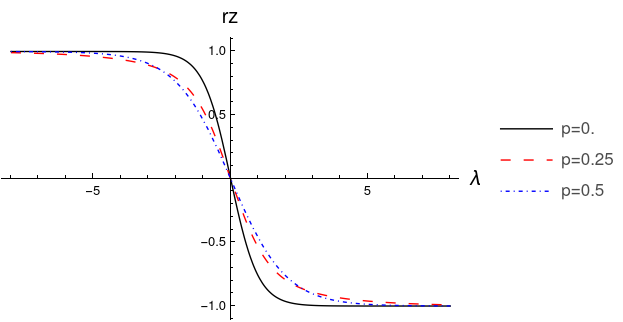
\includegraphics[width=0.6\linewidth]{maxent/figures/rz(lambda)_lambda-8to8.png}
\caption{$r_{z}$ como función de $\lambda$ para diferentes valores de $q$. La apariencia uno a uno sugiere la existencia de una inversa.}
\label{fig:rzinv}
\end{figure}

\subsubsection{Dos soluciones particulares}

Considerando el caso $p=0$ o $p=1$, la ecuación (\ref{eq:RzTanh}) se reduce a 
\begin{equation}
r_z=-\tanh{\lambda}
\end{equation}
de manera que $\lambda=-\text{arctanh}(rz)$.

Si $p=\frac{1}{2}$, la ecuación (\ref{eq:RzTanh}) se reduce a
\begin{equation}
r_z=-\tanh\frac{1}{2}\lambda
\end{equation}
de manera que $\lambda=-\text{arctanh}(2r_{z})$.
En el límite $(1-p)\rightarrow 0$,
\begin{equation}
  r_{z}=-(\tanh{\lambda}+p(\lambda\sech^{2}{\lambda}+\tanh{\lambda}))
\end{equation}
\newpage